%TCIDATA{LaTeXparent=0,0,RUL1.tex}

\begin{biography}[{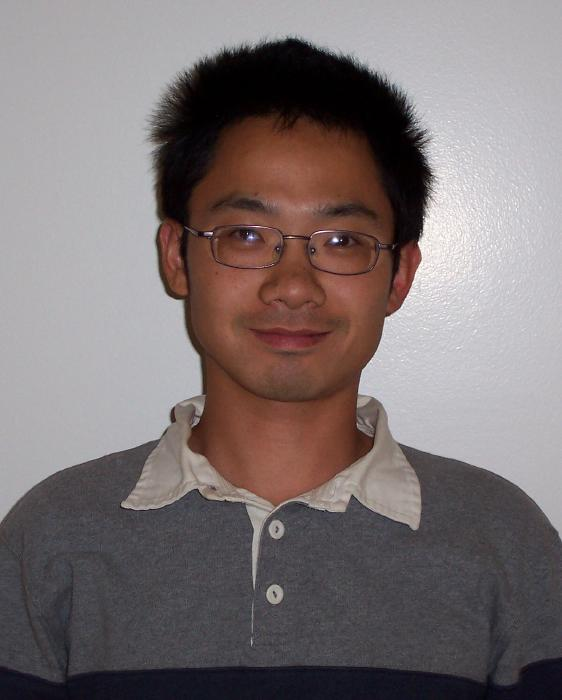
\includegraphics[width=1in,height=1.25in,clip]{BioPhotos/shufang.jpg}}]{David Laredo}
earned his Bachelor of Science from ....
\end{biography}

\begin{biography}[{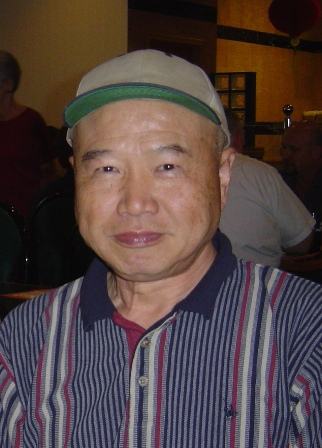
\includegraphics[width=1in,height=1.25in,clip]{BioPhotos/kql.jpg}}]{Zhaoyin Chen}
is an undergraduate student in Computer Science Engineering at University of California, Merced.
\end{biography}

\begin{biography}[{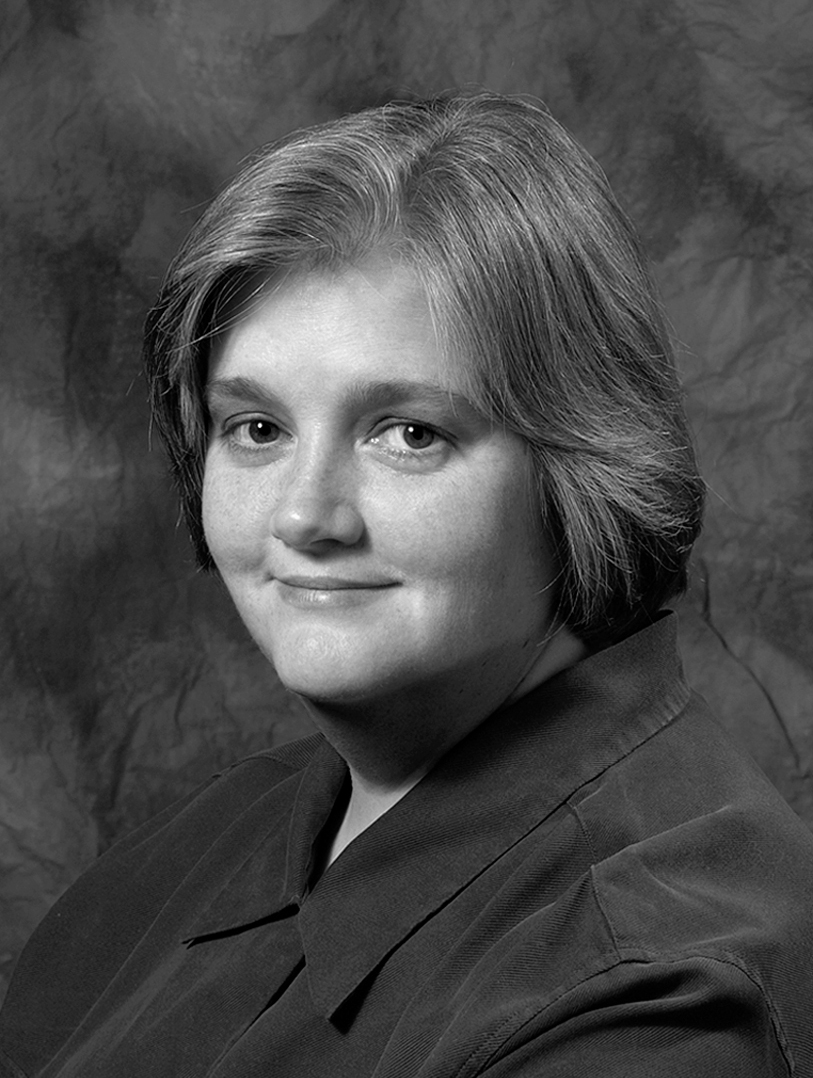
\includegraphics[width=1in,height=1.25in,clip]{BioPhotos/kr.jpg}}]{Oliver Sch\"utze}
earned her Master of Science in Physical Therapy from Boston University in 1989 and her PhD in Biomechanics and Movement Sciences from the University of Delaware in 1998.  Dr. Rudolph joined the faculty of the Department of Physical Therapy and Program in Biomechanics and Movement Sciences at the University of Delaware in 1999 and is currently an Assistant Professor.  She has served as a manuscript reviewer for the Journal of Orthopaedic and Sports Physical Therapy, Archives of Physical Medicine and Rehabilitation, Journal of Applied Biomechanics and the European Journal of Applied Physiology and has reviewed grants for the National Institutes of Health Musculoskeletal and Rehabilitation Sciences Study section. Dr. Rudolph's research interests include analysis of walking in patients with knee osteoarthritis and neurological injury and development of research based physical therapy interventions.
\end{biography}


\begin{biography}[{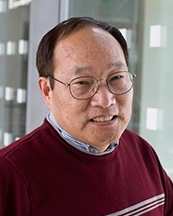
\includegraphics[width=1in,height=1.25in,clip]{BioPhotos/jqs.jpg}}]{Jian-Qiao Sun}
earned a BS degree in Solid Mechanics from Huazhong University of Science and Technology in 1982, and PhD in Mechanical Engineering from University of California at Berkeley in 1988.  In 1994, Dr. Sun joined the faculty of the department of Mechanical Engineering at the University of Delaware as an Assistant Professor, was promoted to Associate Professor in 1998 and to Professor in 2003.  Dr. Sun joined the new campus of University of California at Merced in 2007 and is currently Professor and Chair of Mechanical Engineering. He serves as the Editor-in-Chief of the International Journal of Dynamics and Control by Springer.  His research interests include random vibrations, nonlinear controls, energy harvesting technologies, and data-driven modeling and analysis of complex mechanical systems.
\end{biography}


